\documentclass[11pt, a4paper]{article}
\usepackage{pdfpages}
\usepackage{parallel}
\usepackage[T2A]{fontenc}
\usepackage{ucs}
\usepackage[utf8x]{inputenc}
\usepackage[polish,english,russian]{babel}
\usepackage{hyperref}
\usepackage{rotating}
\usepackage[inner=2cm,top=1.8cm,outer=2cm,bottom=2.3cm,nohead]{geometry}
\usepackage{listings}
\usepackage{graphicx}
\usepackage{wrapfig}
\usepackage{longtable}
\usepackage{indentfirst}
\usepackage{array}
\usepackage{tikzsymbols}
\usepackage{soul}
\usepackage[ruled,vlined]{algorithm2e}
%\counterwithout{figure}{section} 

\usepackage{url}
\makeatletter
\g@addto@macro{\UrlBreaks}{\UrlOrds}
\makeatother

\newcolumntype{P}[1]{>{\raggedright\arraybackslash}p{#1}}
\frenchspacing
\usepackage{fixltx2e} %text sub- and superscripts
\usepackage{icomma} % коскі ў матэматычным рэжыме
\PreloadUnicodePage{4}

\newcommand{\longpage}{\enlargethispage{\baselineskip}}
\newcommand{\shortpage}{\enlargethispage{-\baselineskip}}

\def\switchlang#1{\expandafter\csname switchlang#1\endcsname}
\def\switchlangbe{
\let\saverefname=\refname%
\def\refname{Літаратура}%
\def\figurename{Іл.}%
}
\def\switchlangen{
\let\saverefname=\refname%
\def\refname{References}%
\def\figurename{Fig.}%
}
\def\switchlangru{
\let\saverefname=\refname%
\let\savefigurename=\figurename%
\def\refname{Литература}%
\def\figurename{Рис.}%
}

\hyphenation{admi-ni-stra-tive}
\hyphenation{ex-pe-ri-ence}
\hyphenation{fle-xi-bi-li-ty}
\hyphenation{Py-thon}
\hyphenation{ma-the-ma-ti-cal}
\hyphenation{re-ported}
\hyphenation{imp-le-menta-tions}
\hyphenation{pro-vides}
\hyphenation{en-gi-neering}
\hyphenation{com-pa-ti-bi-li-ty}
\hyphenation{im-pos-sible}
\hyphenation{desk-top}
\hyphenation{elec-tro-nic}
\hyphenation{com-pa-ny}
\hyphenation{de-ve-lop-ment}
\hyphenation{de-ve-loping}
\hyphenation{de-ve-lop}
\hyphenation{da-ta-ba-se}
\hyphenation{plat-forms}
\hyphenation{or-ga-ni-za-tion}
\hyphenation{pro-gramming}
\hyphenation{in-stru-ments}
\hyphenation{Li-nux}
\hyphenation{sour-ce}
\hyphenation{en-vi-ron-ment}
\hyphenation{Te-le-pathy}
\hyphenation{Li-nux-ov-ka}
\hyphenation{Open-BSD}
\hyphenation{Free-BSD}
\hyphenation{men-ti-on-ed}
\hyphenation{app-li-ca-tion}

\def\progref!#1!{\texttt{#1}}
\renewcommand{\arraystretch}{2} %Іначай формулы ў матрыцы зліпаюцца з лініямі
\usepackage{array}

\def\interview #1 (#2), #3, #4, #5\par{

\section[#1, #3, #4]{#1 -- #3, #4}
\def\qname{LVEE}
\def\aname{#1}
\def\q ##1\par{{\noindent \bf \qname: ##1 }\par}
\def\a{{\noindent \bf \aname: } \def\qname{L}\def\aname{#2}}
}

\def\interview* #1 (#2), #3, #4, #5\par{

\section*{#1\\{\small\rm #3, #4. #5}}
\ifx\ParallelWhichBox\undefined%
    \addcontentsline{toc}{section}{#1, #3, #4}%
\else%
\ifnum\ParallelWhichBox=0%
    \addcontentsline{toc}{section}{#1, #3, #4}%
\fi\fi%

\def\qname{LVEE}
\def\aname{#1}
\def\q ##1\par{{\noindent \bf \qname: ##1 }\par}
\def\a{{\noindent \bf \aname: } \def\qname{L}\def\aname{#2}}
}

\newcommand{\interviewfooter}[1]{
\vskip 1em
\noindent \textit{#1}
}

\switchlang{en}
\begin{document}

\title{1993 "--- Colani Trackball}
\date{}
\maketitle
\selectlanguage{english}
Apparently, the  Colani Trackball was, along with the mouse of the same name, the first among the so-called “designer” mice - devices officially developed in collaboration with celebrities in the field of technical design. This mouse was named and shaped by Luigi Colani \cite{wiki}.

\textit{Colani is best known in the automotive industry, with about 40 concept cars; no less actively he designed furniture, household items, household appliances. And Luigi Colani's fruitful collaboration with the German company Vobis Microcomputer, the owner of the Highscreen trademark, led to the release of several personal computers, joysticks, mice and trackballs based on his design.}

\begin{figure}[h]
    \centering
    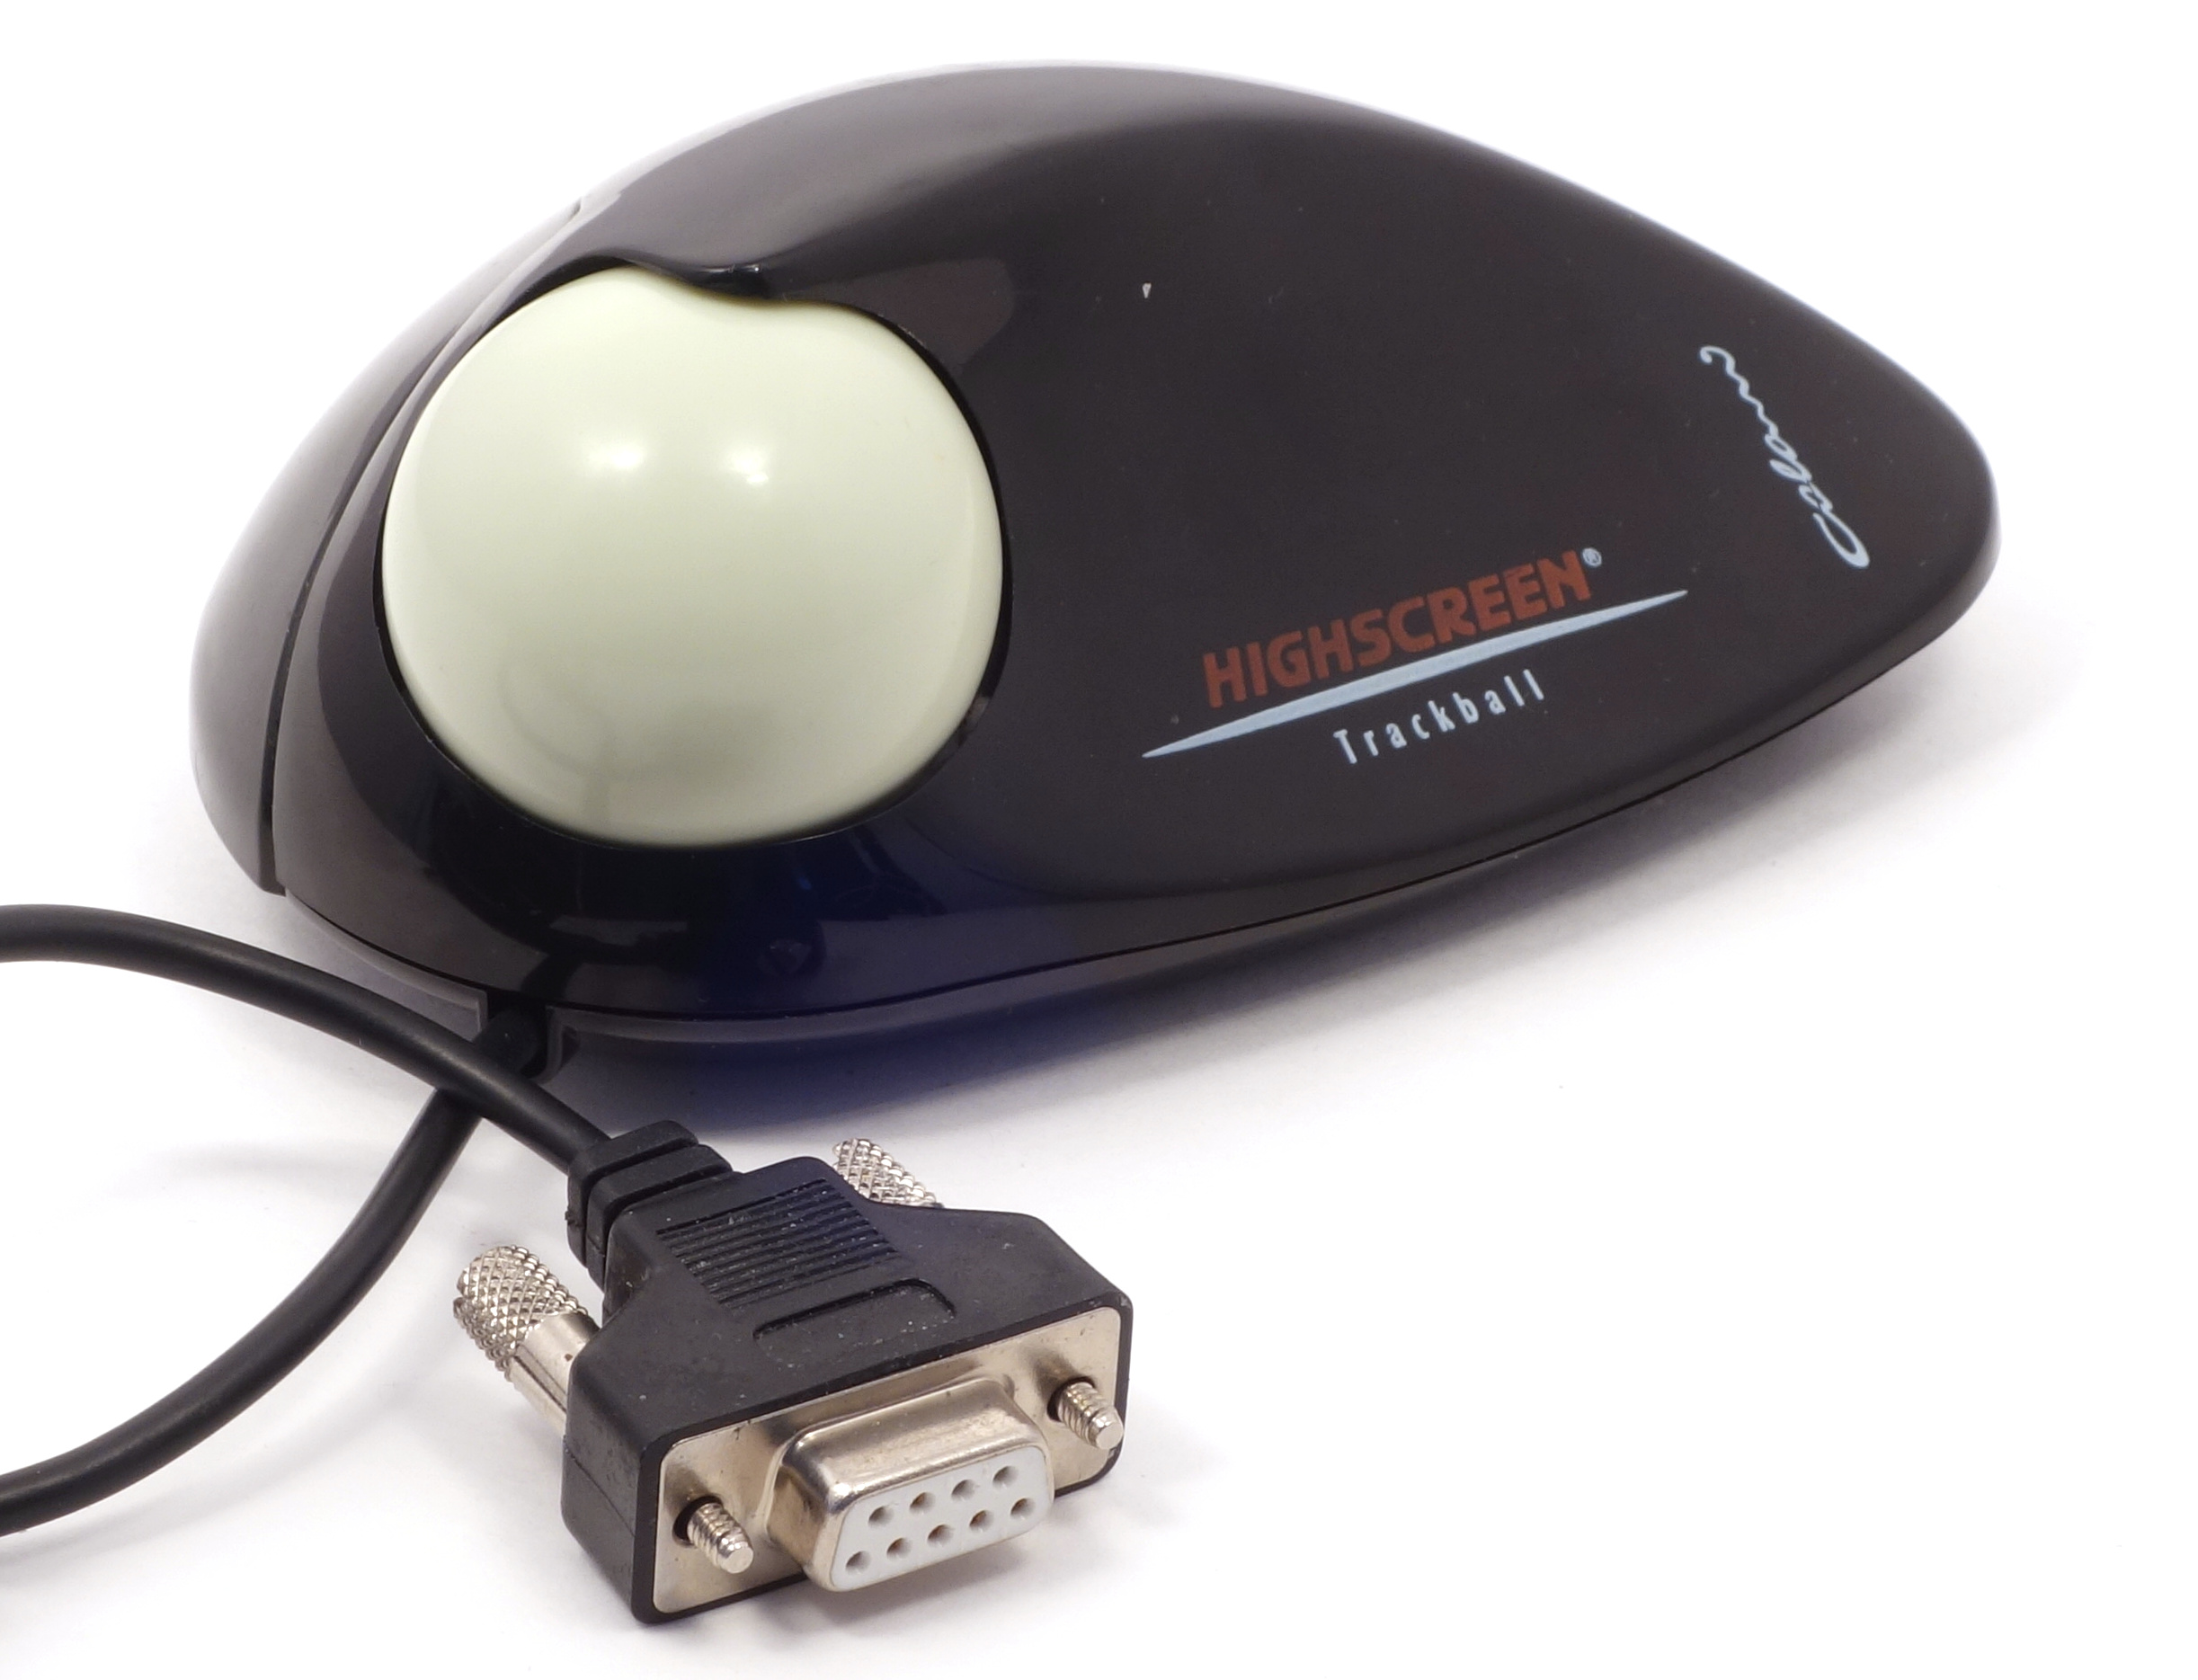
\includegraphics[scale=0.475]{1993_colani_trackball/pic_b_60.jpg}
    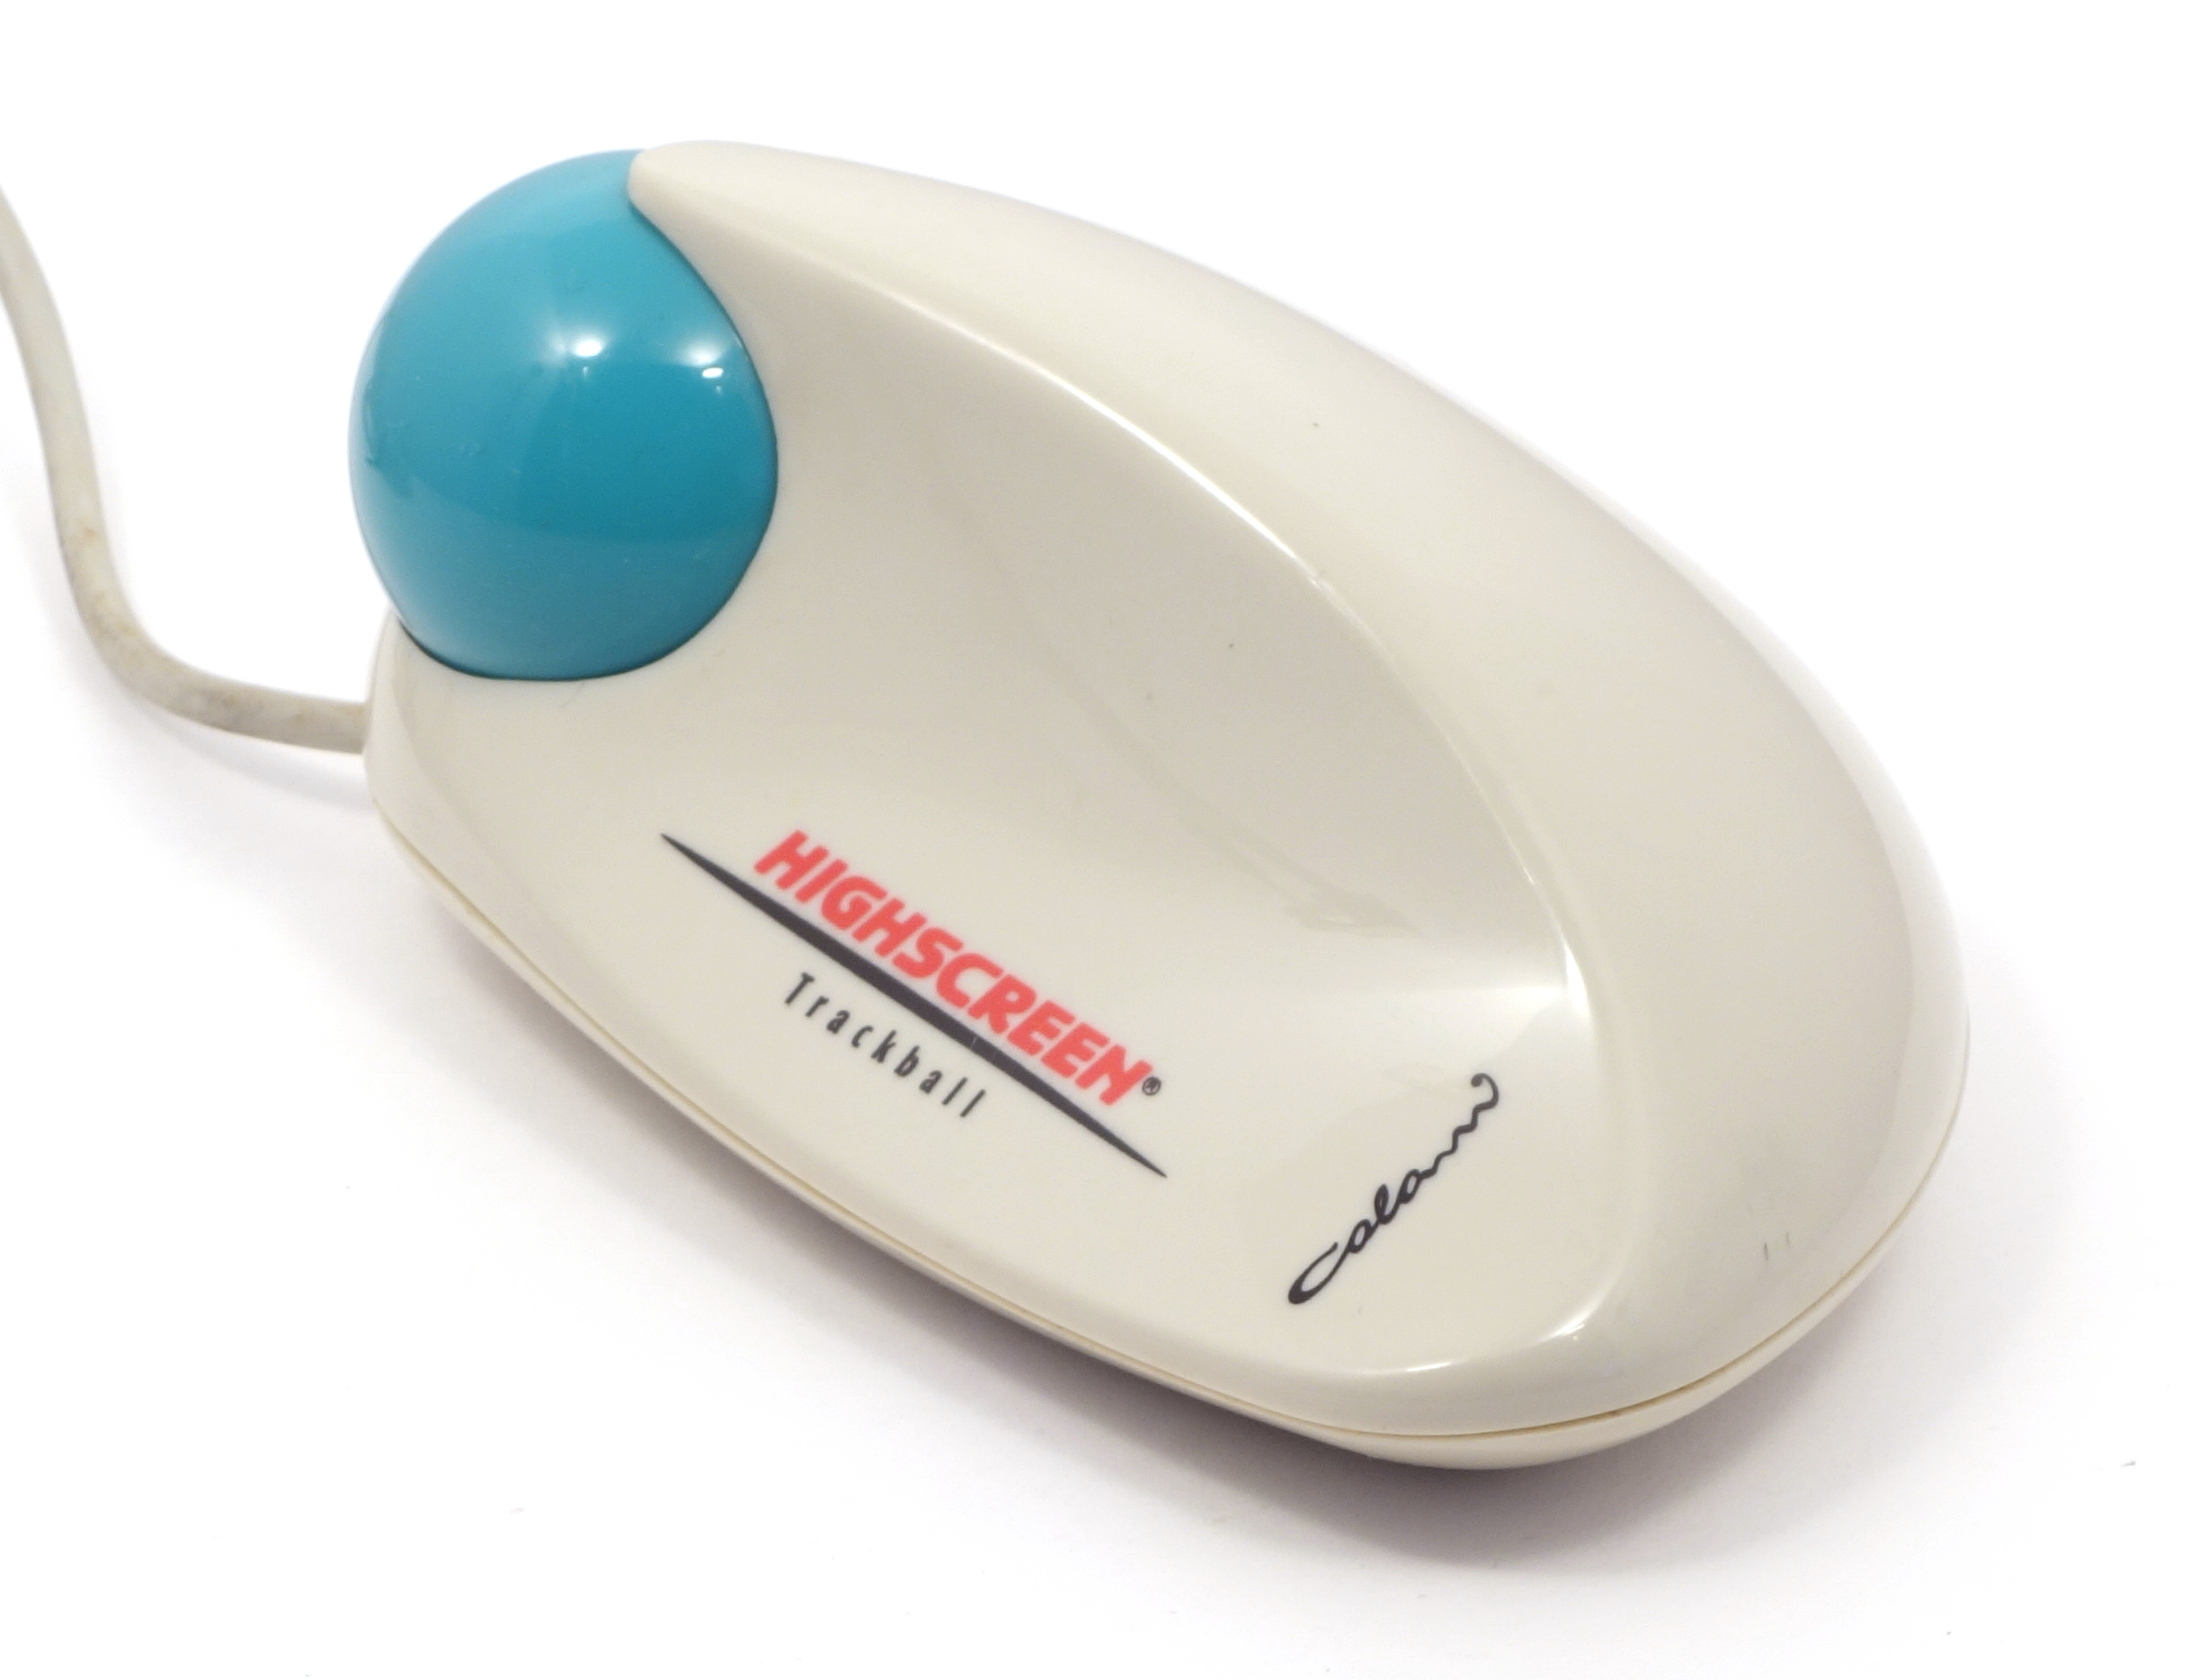
\includegraphics[scale=0.475]{1993_colani_trackball/pic_w_60.jpg}
    \caption{Colani Trackball}
    \label{fig:ColaniPic}
\end{figure}

The HIGHSCREEN Colani Trackball shown in figure \ref{fig:ColaniPic} is representative of this line. This trackball model (together with a similarly designed Colani Mouse from the same manufacturer) won the prestigious “IF Design Award” from iF International Forum Design GmbH in 1993 \cite{award}.

Starting with concept cars that emphasized the aerodynamics of high speeds, Luigi Colani developed his own new style of industrial design, in the direction now known as bionics. The main principle of bionics is to give objects roundness and streamlined natural forms (figure \ref{fig:ColaniTopBottom}).

{According to the researchers of Luigi Colani's work, in general, the designer recognized the primacy of the object's function over its form. However, time after time, he could not resist the opportunity to make the product more “natural”, to provide it with curves, sometimes turning into each other in the most unexpected way, which suggests thoughts of rocks altered by the long work of wind or waves. In conservative industries, such as the automotive industry, this approach was perceived as too eccentric.}

~

\begin{figure}[h]
    \centering
    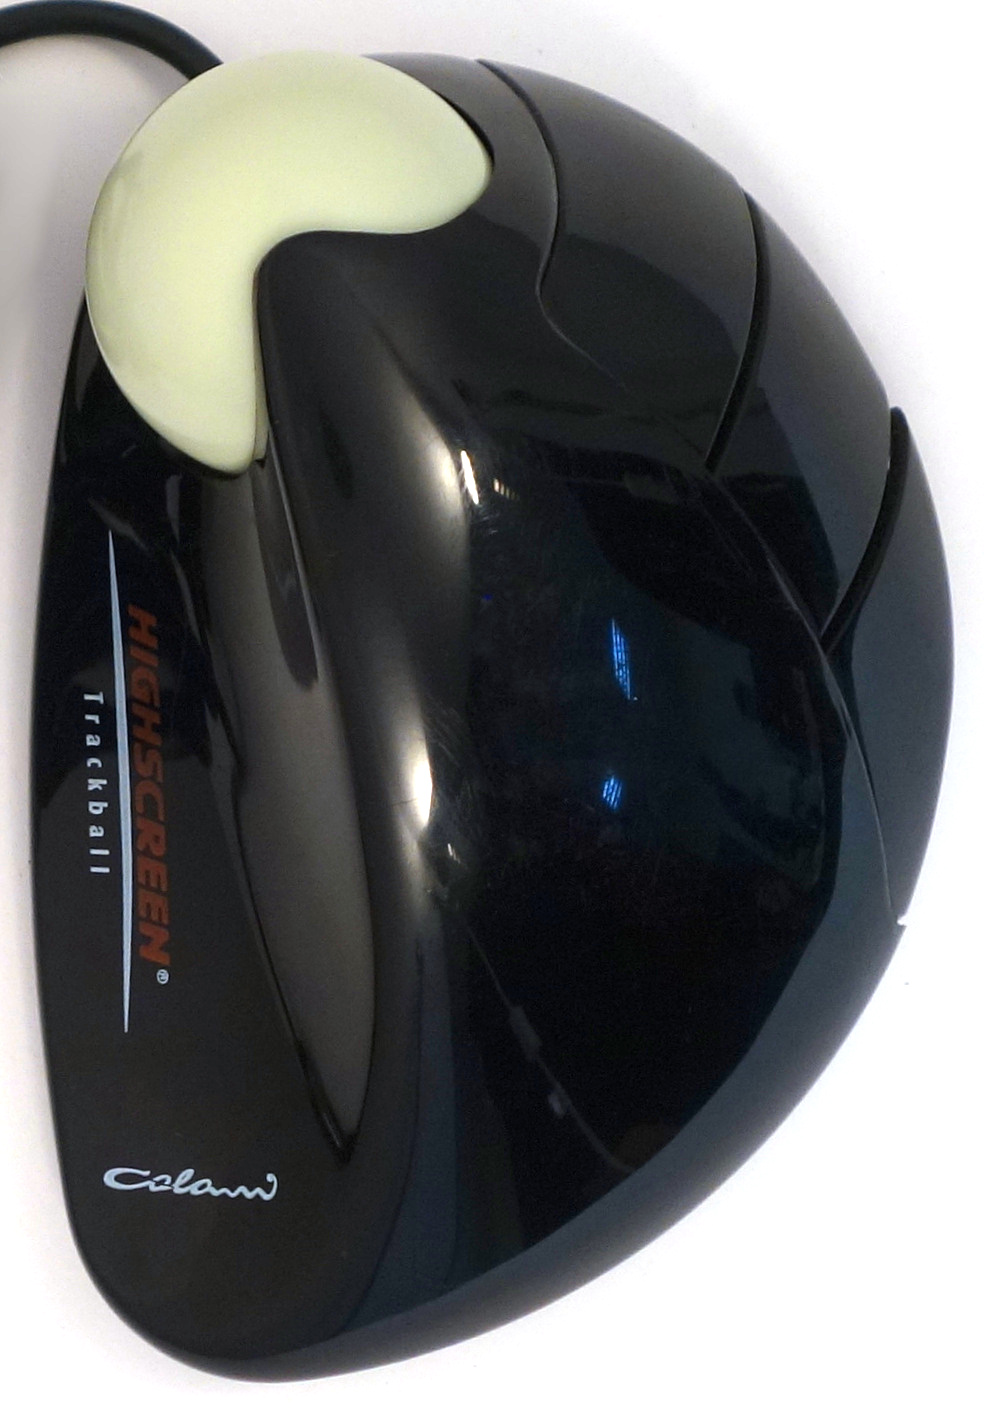
\includegraphics[scale=0.51]{1993_colani_trackball/top_b_30.jpg}
    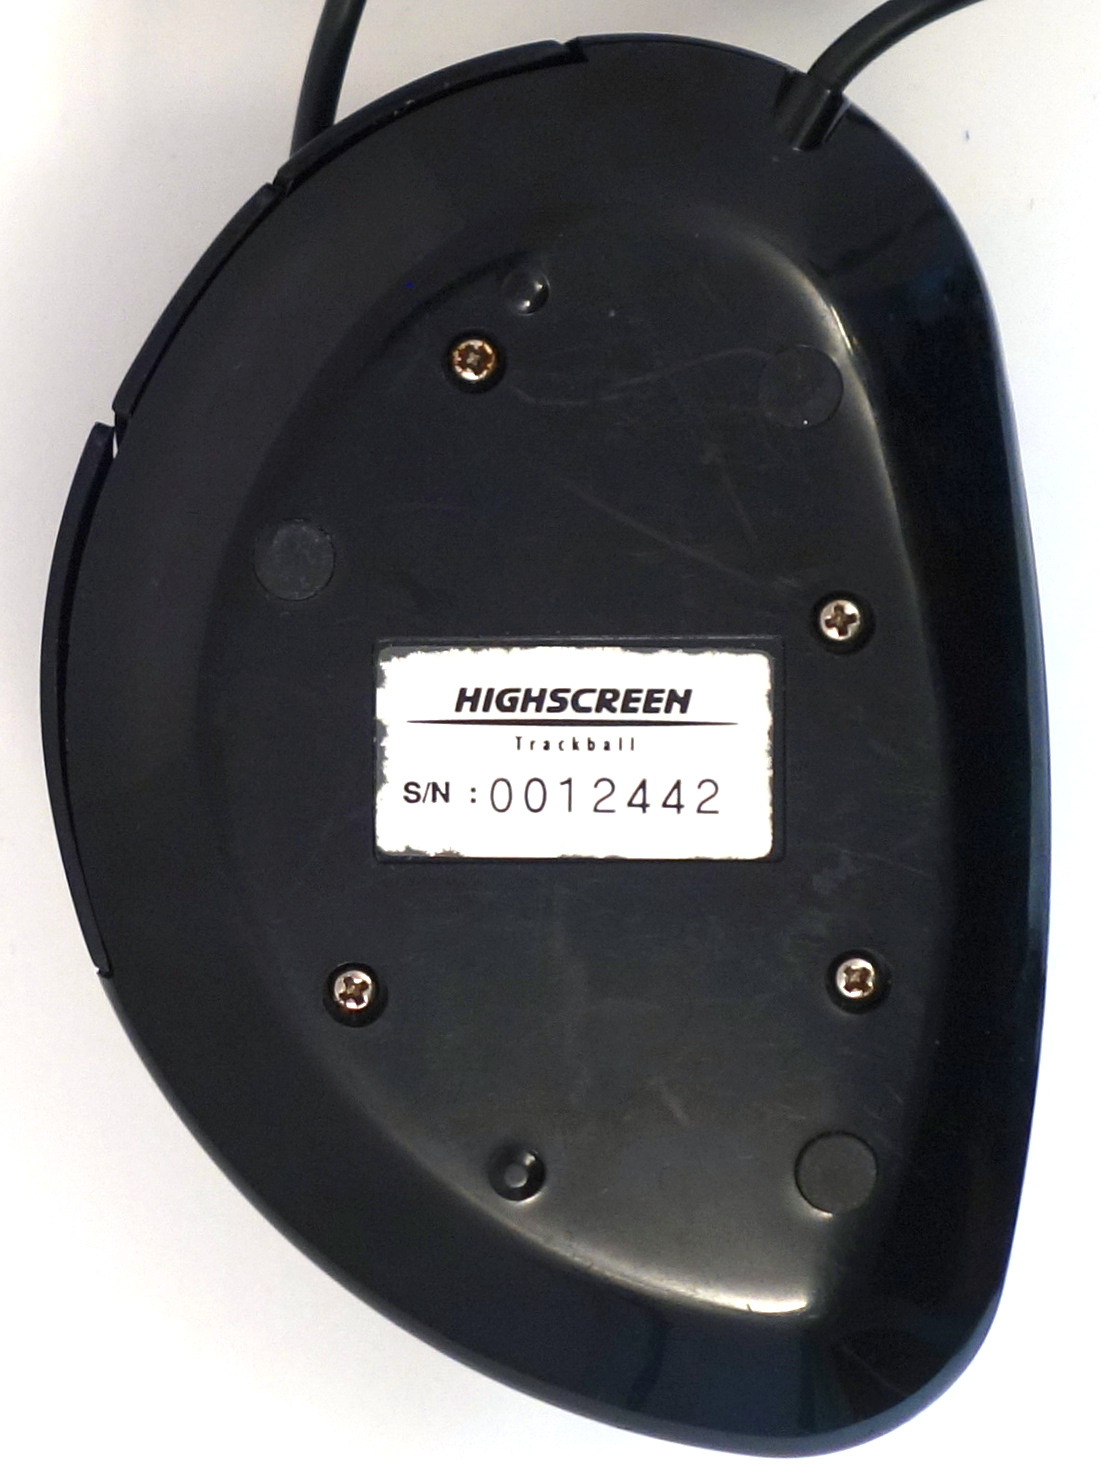
\includegraphics[scale=0.51]{1993_colani_trackball/bottom_b_30.jpg}
    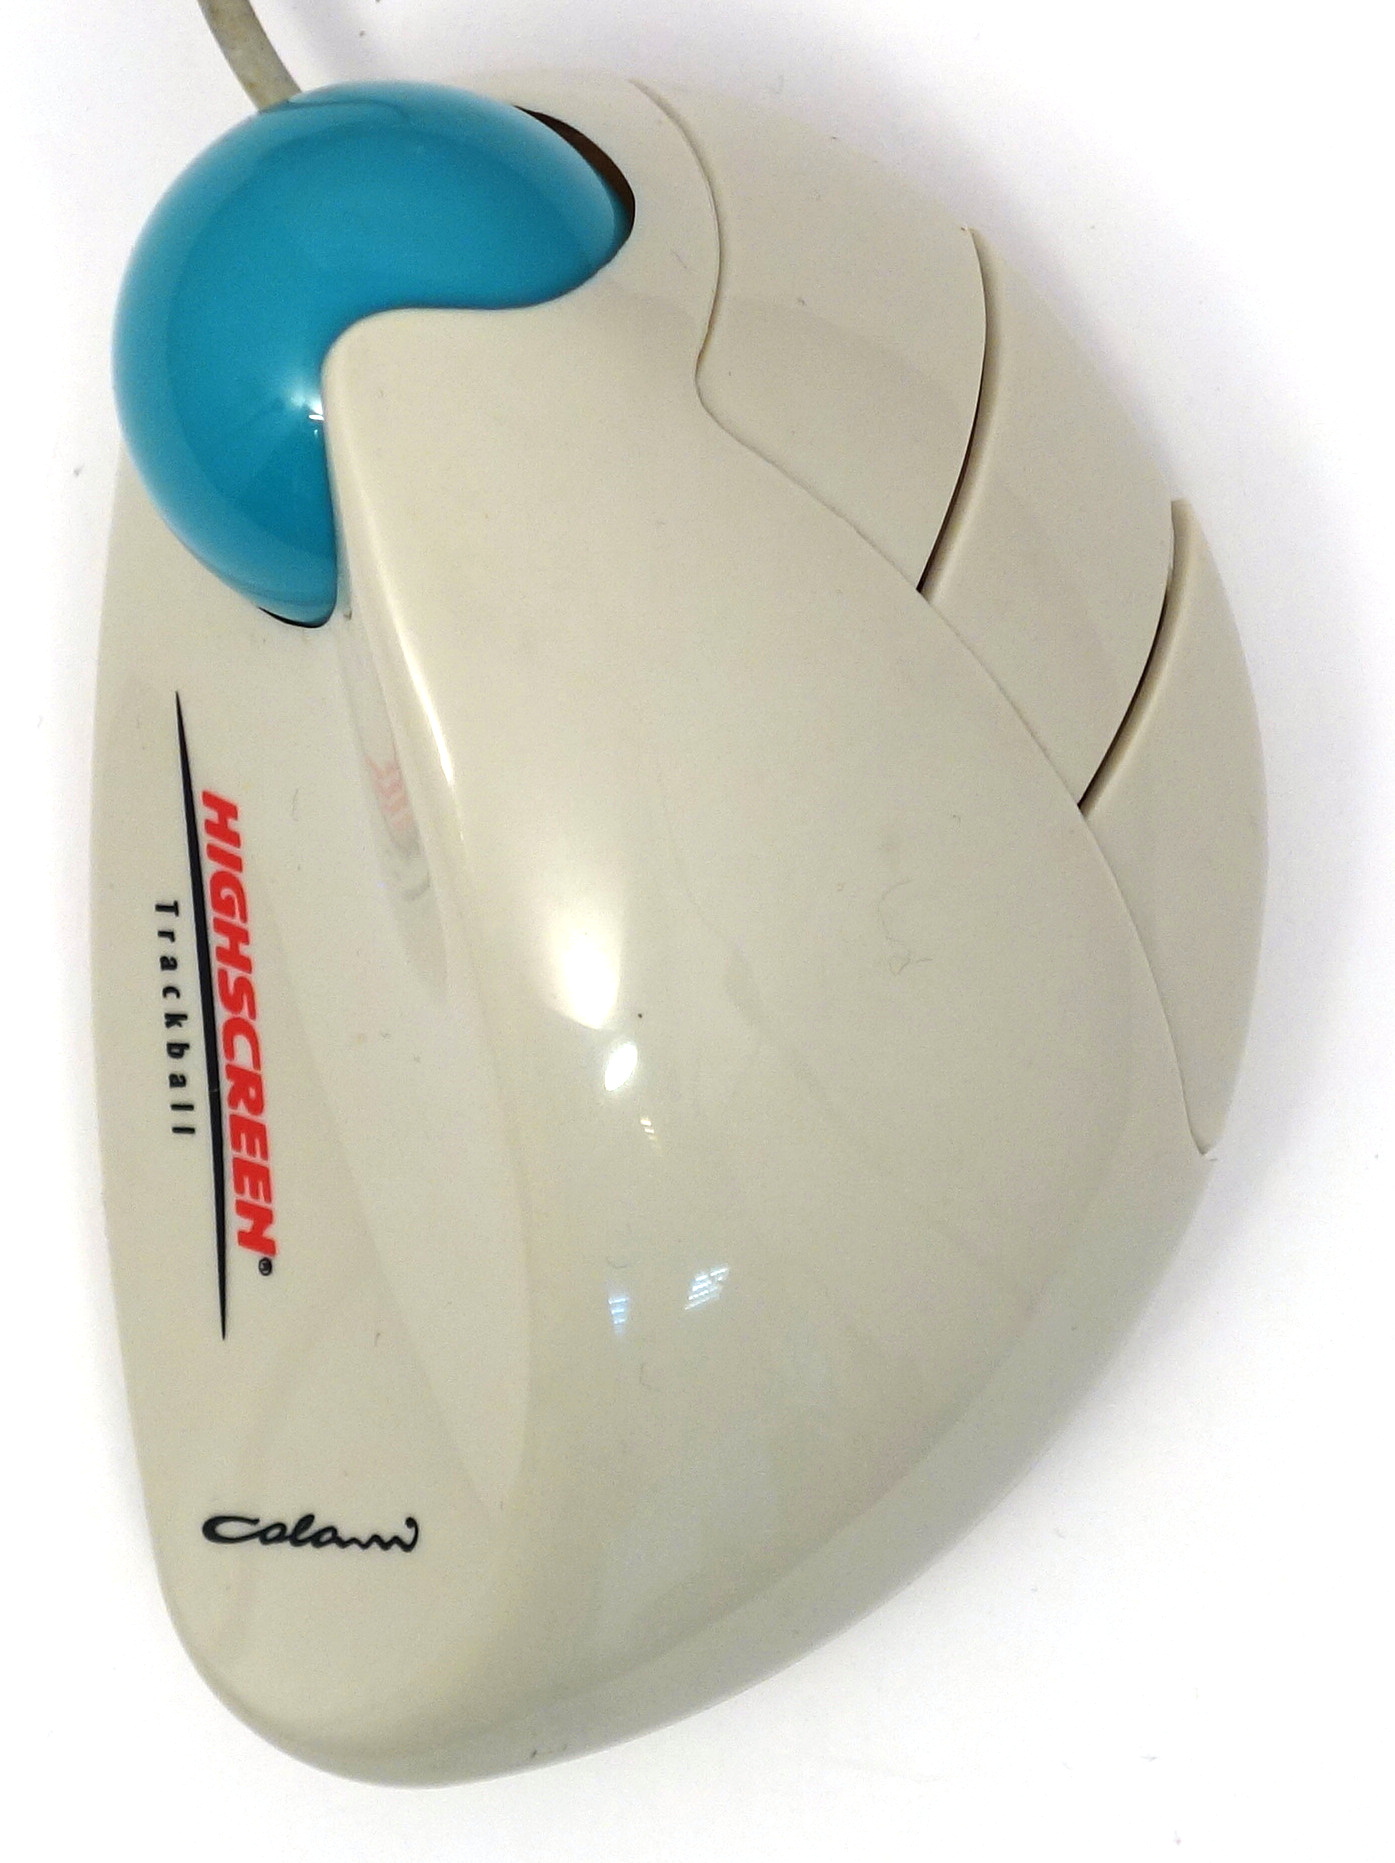
\includegraphics[scale=0.41]{1993_colani_trackball/top_w_30.jpg}
    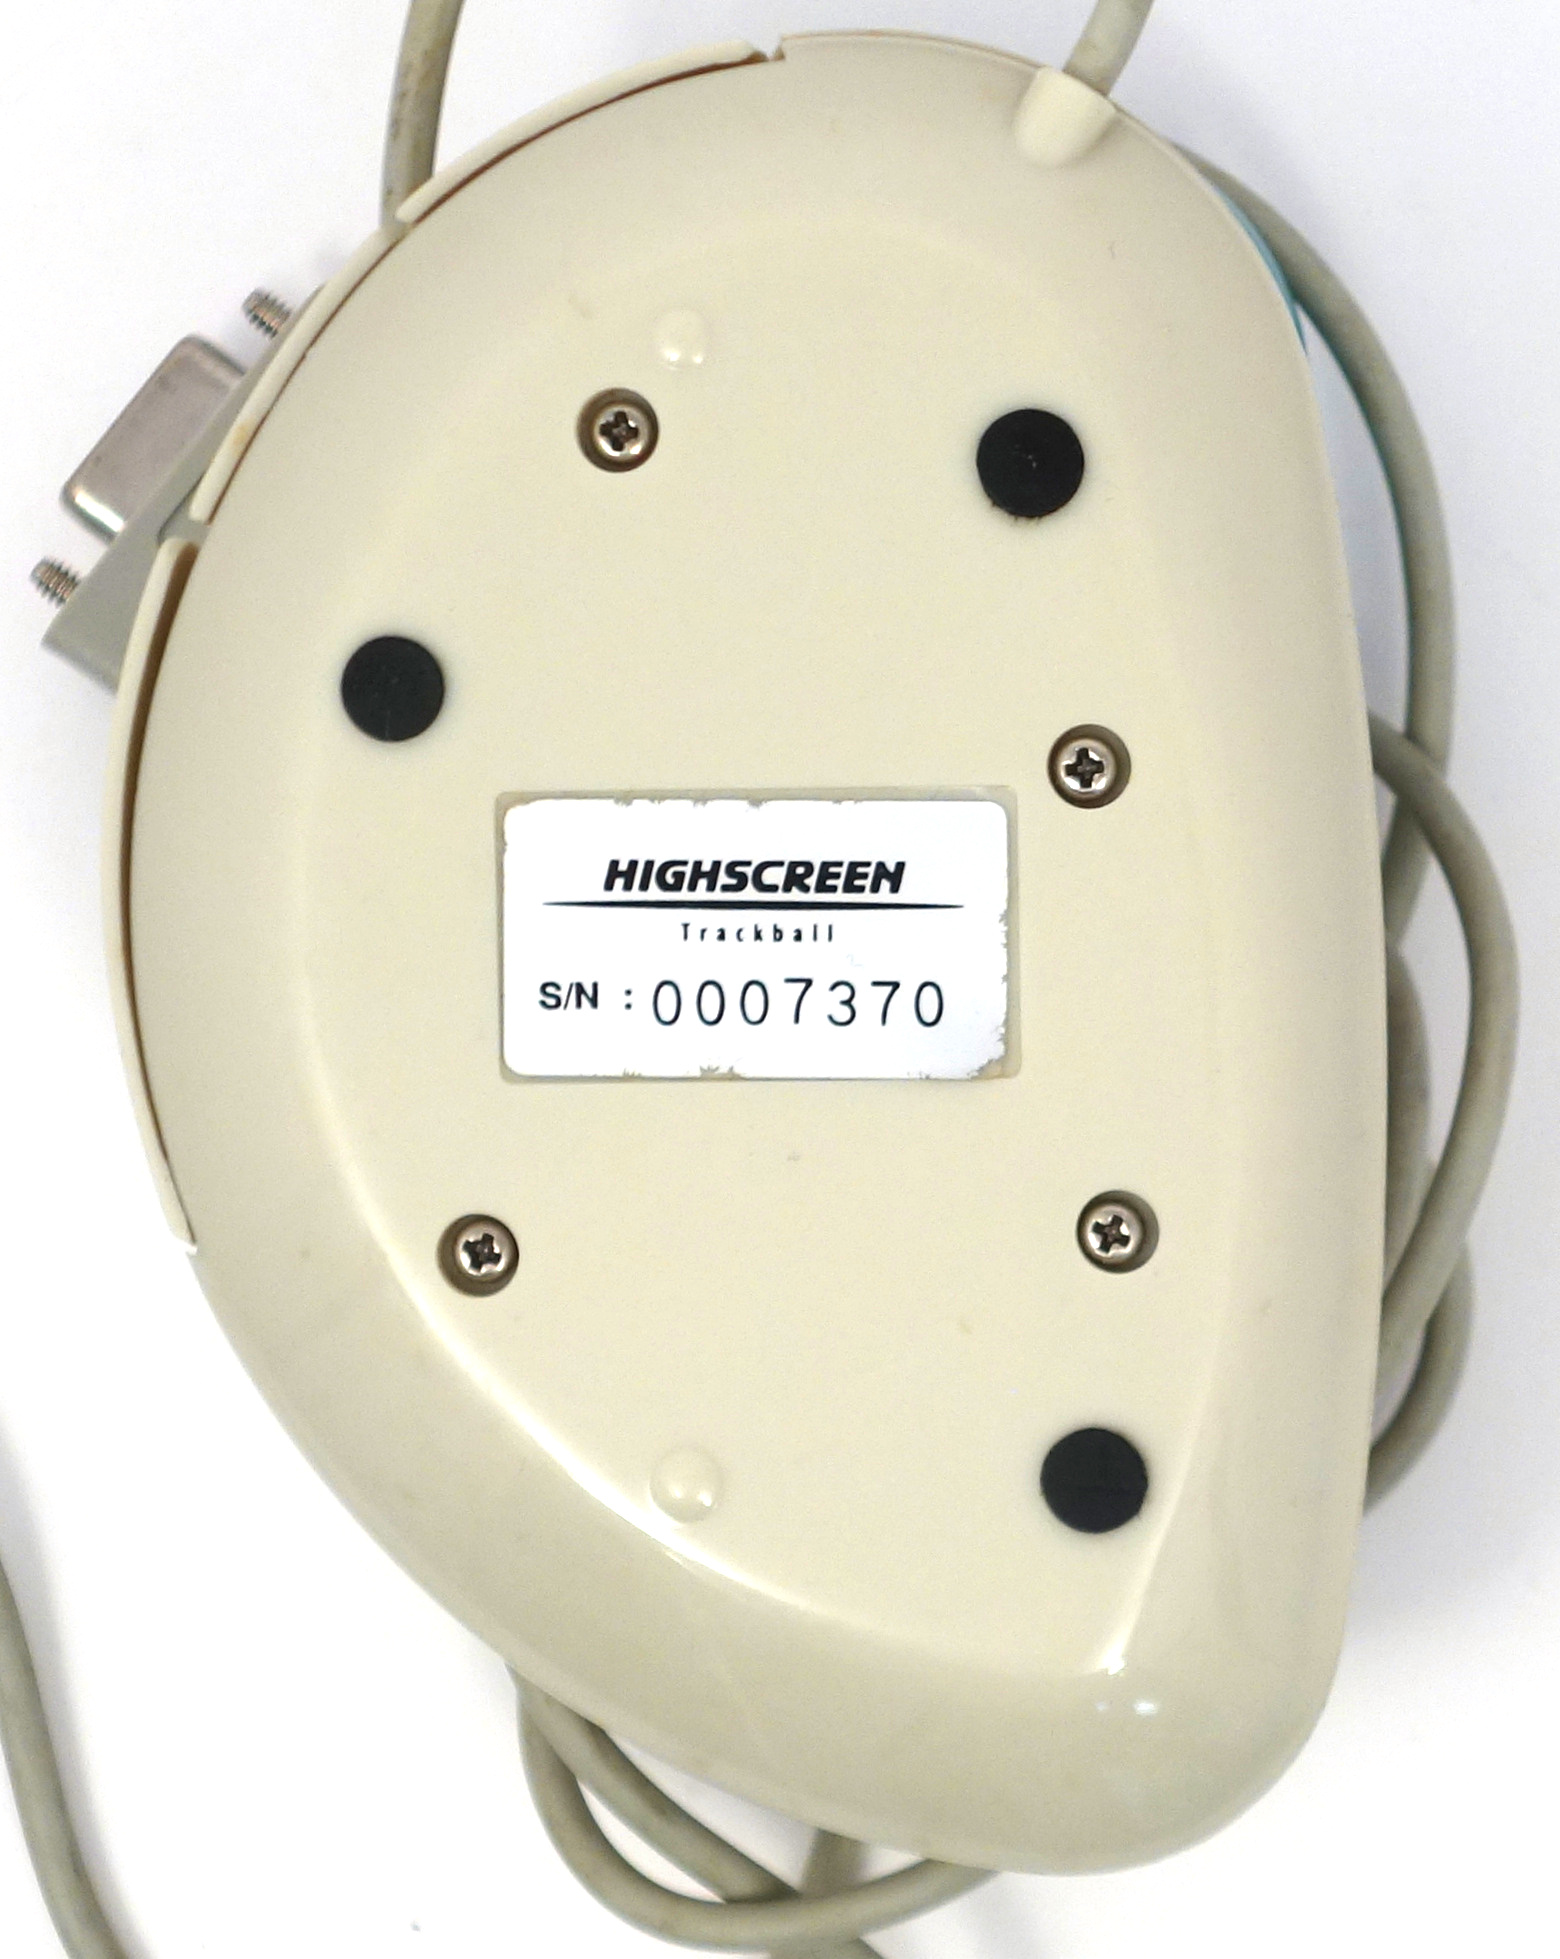
\includegraphics[scale=0.4]{1993_colani_trackball/bottom_w_30.jpg}
    \caption{Colani Trackball, top and bottom views}
    \label{fig:ColaniTopBottom}
\end{figure}

~

However, with regard to cursor controls, the designer turned out to be the forerunner of the era of ergonomic mice that came after some time with a complex asymmetrical shape that provides the most comfortable position for the human hand. This trend was promoted both by the fact that such forms are easily reproduced when casting plastic bodies of manipulators (which cannot be said, for example, about car bodies), and the popularity of clay models with traces of a hand squeezing them, which allowed the developer to obtain an anatomically accurate and unusual outwardly product without special difficulties. However, judging by some signs, Luigi Colani himself did not resort to this method of shaping.

As you can see in figures \ref{fig:ColaniSize} and \ref{fig:ColaniHand}, the Colani Trackball is a very compact product that fits almost entirely in the palm of your hand.

\begin{figure}[h]
    \centering
    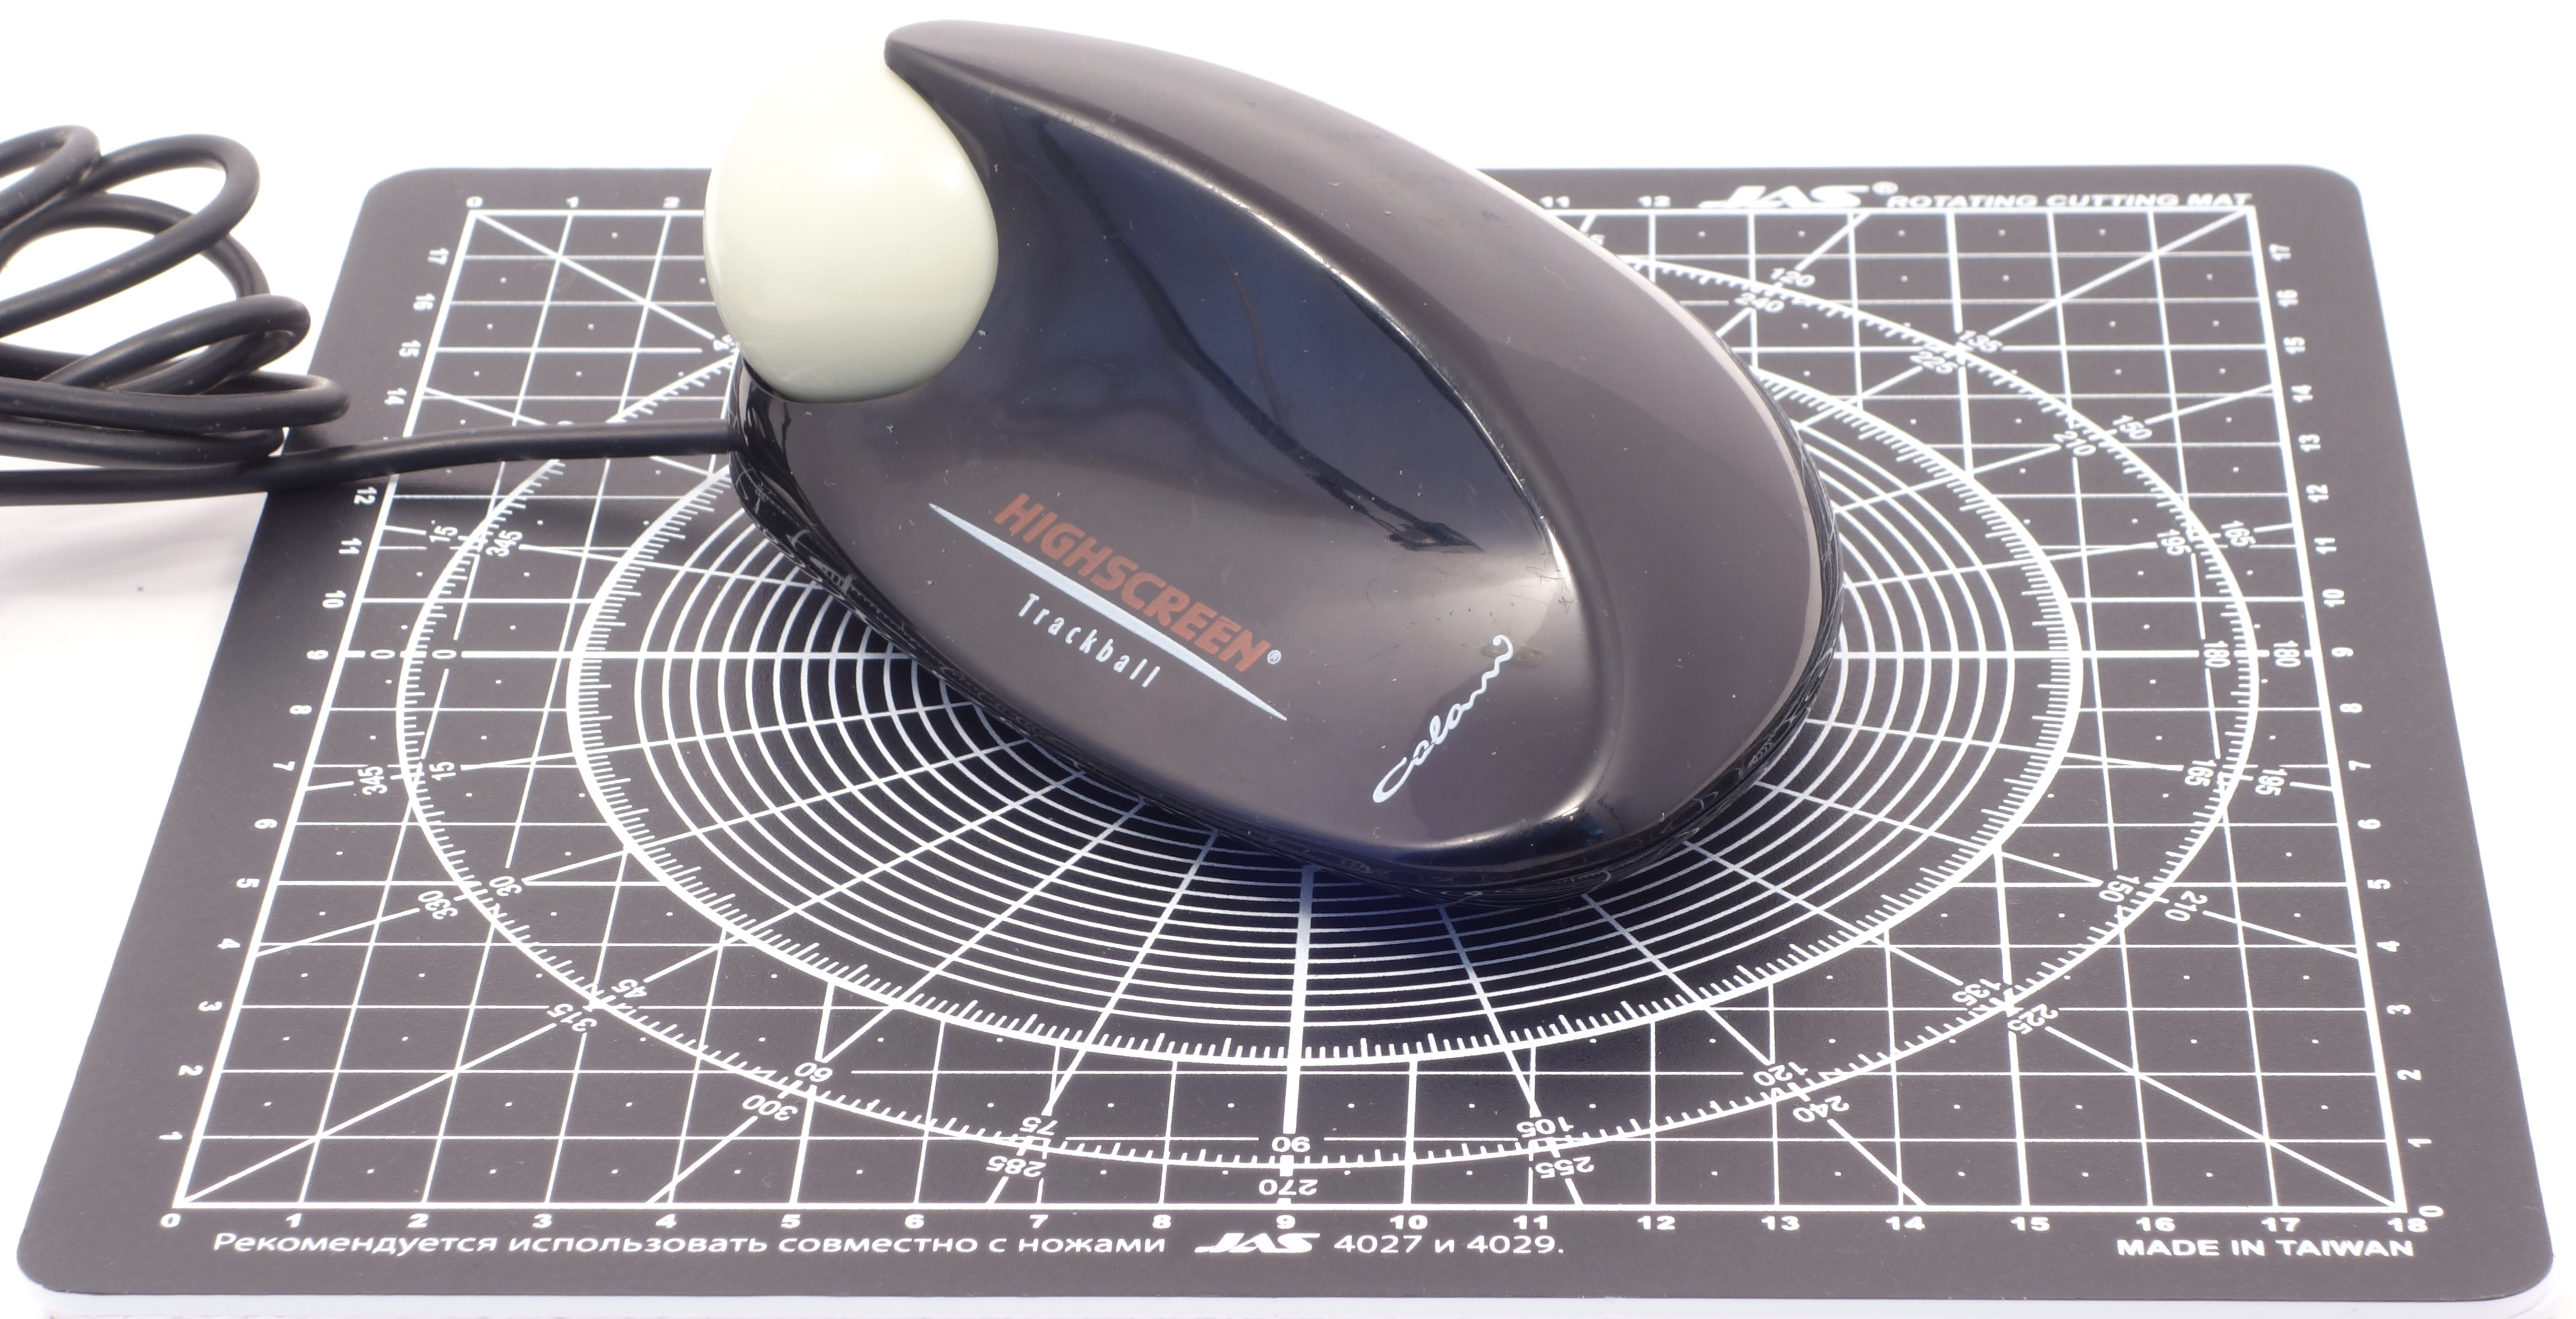
\includegraphics[scale=0.52]{1993_colani_trackball/size_30.jpg}
    \caption{Colani Trackball on a graduated pad with a grid step of 1~cm}
    \label{fig:ColaniSize}
\end{figure}

The concave part of the body practically does not work as a support for the hand, but mainly has an aesthetic and artistic function (which, by the way, can be said about the vast majority of designer manipulators). However, in general, the position of the hand on the trackball is comfortable, the keys are easy to reach and have sufficient area, and the ball protrudes significantly from the body, thus being very convenient to rotate (of course, if the user is able to reach it).

~

\begin{figure}[h]
    \centering
    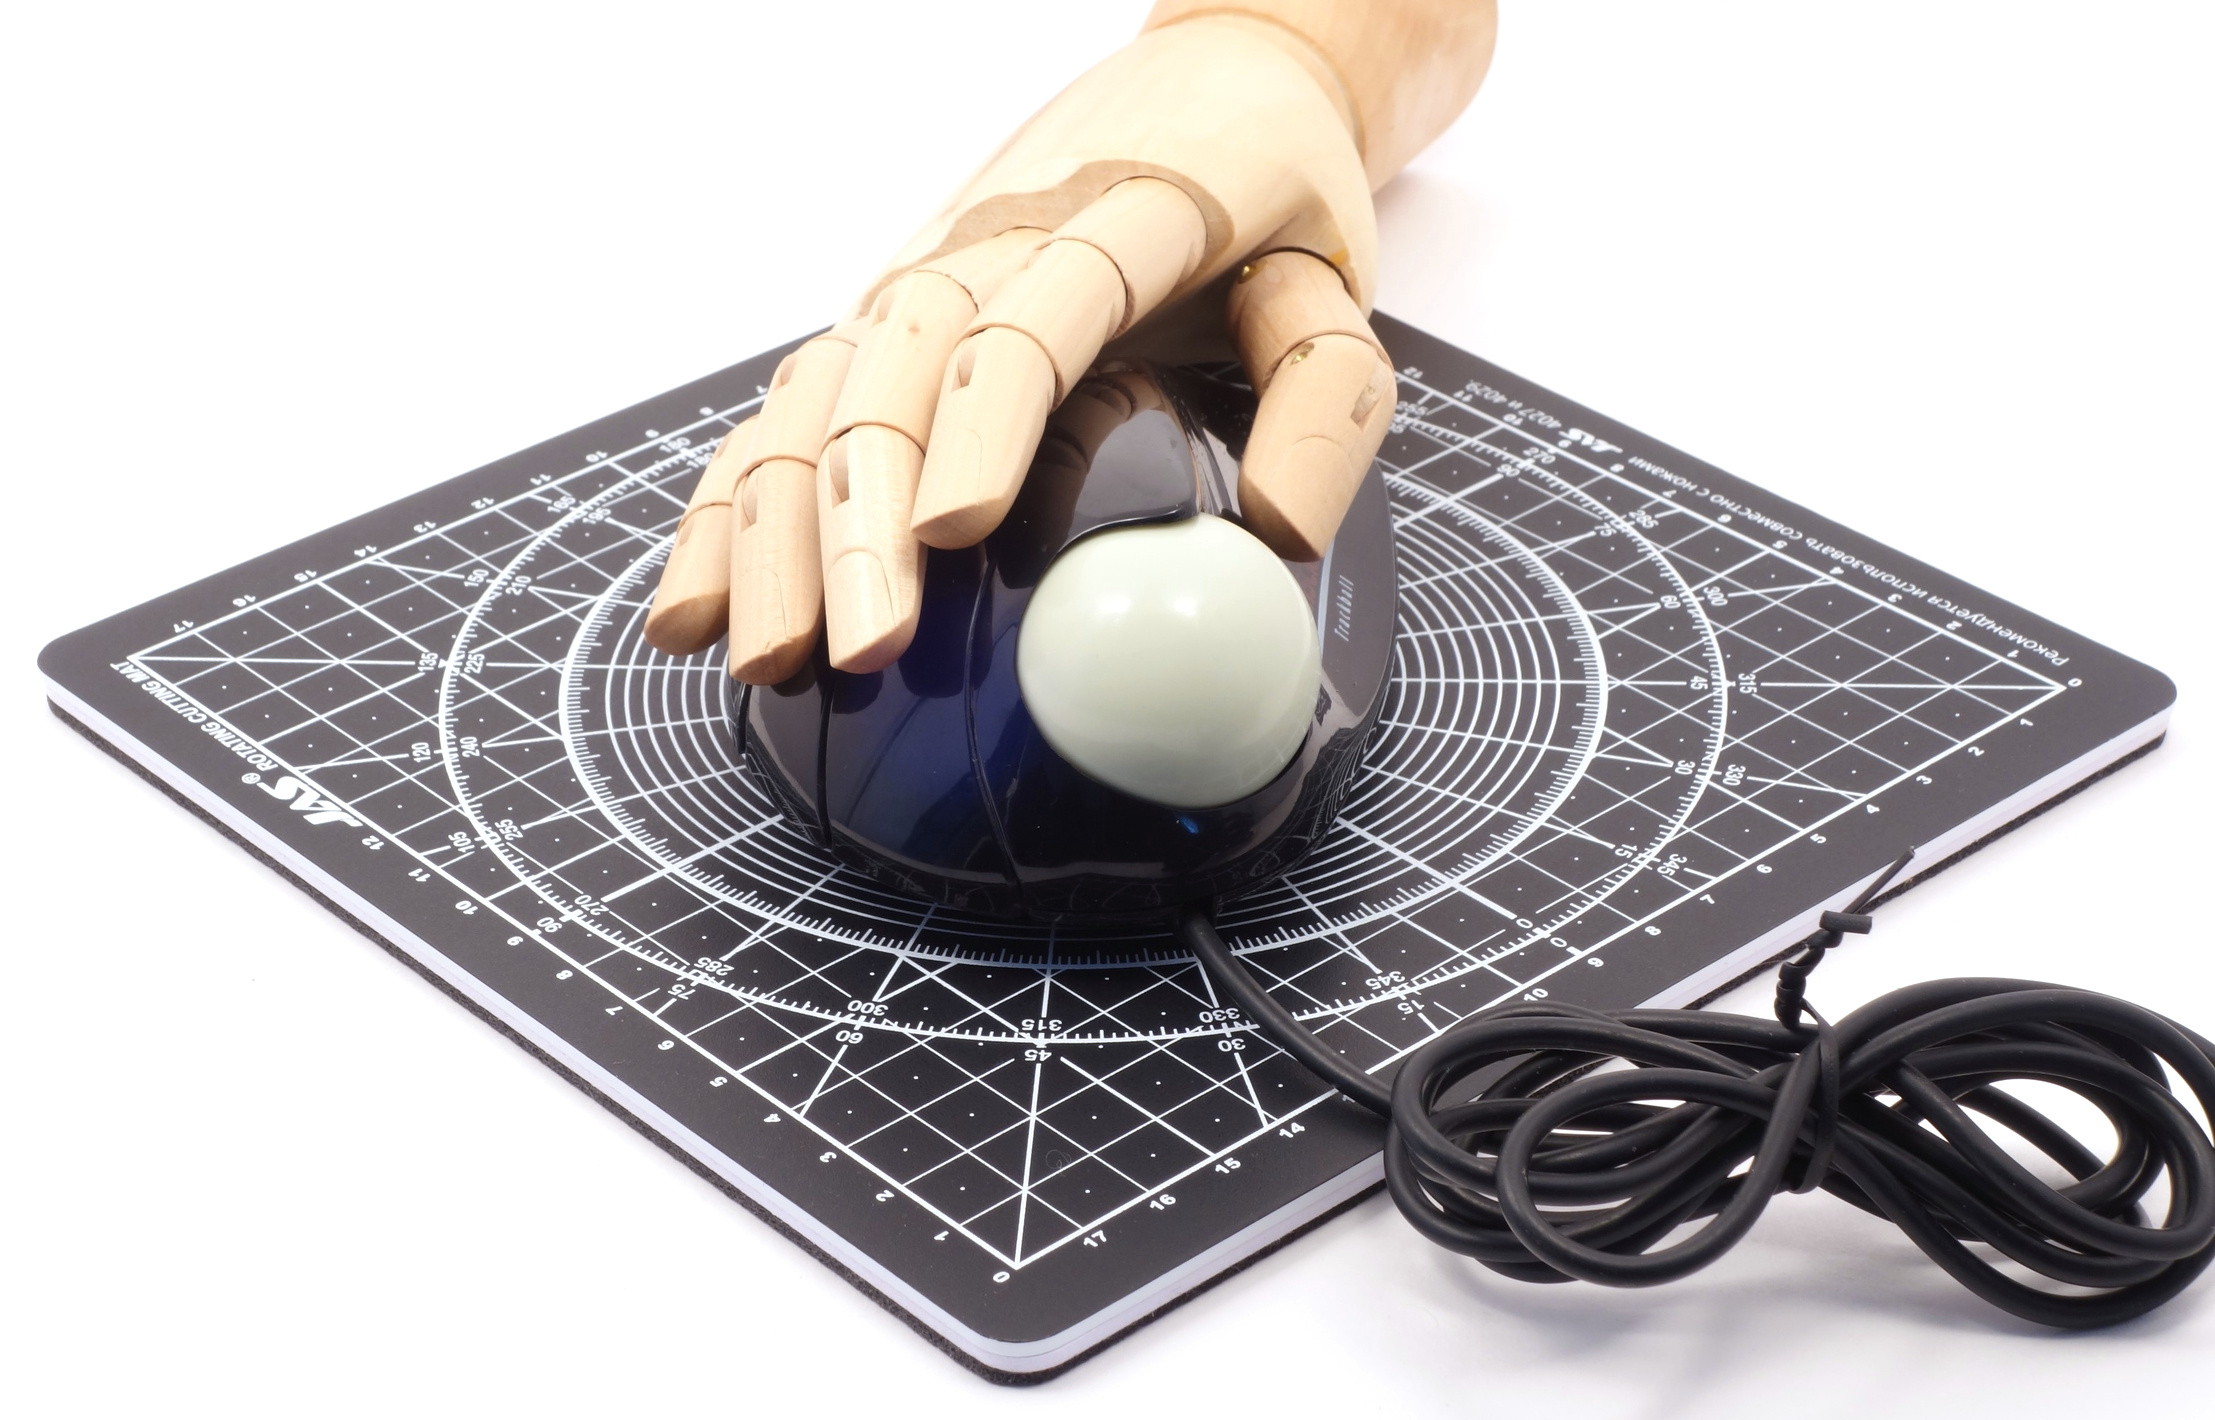
\includegraphics[scale=0.15]{1993_colani_trackball/hand_60.jpg}
    \caption{Colani Trackball with a human hand model}
    \label{fig:ColaniHand}
\end{figure}

Trackball internals are shown on figure \ref{fig:ColaniInside}. This is an opto-mechanical device with toothed disks of encoders, typical for the late 80s and early 90s. Note that the choice of details is extremely budgetary: trackball contains a bare minimum of movable parts and a bare minimum of metal elements (only axes of encoders, a clamping spring and a metal plate located under the printed circuit board).

\begin{figure}[h]
    \centering
    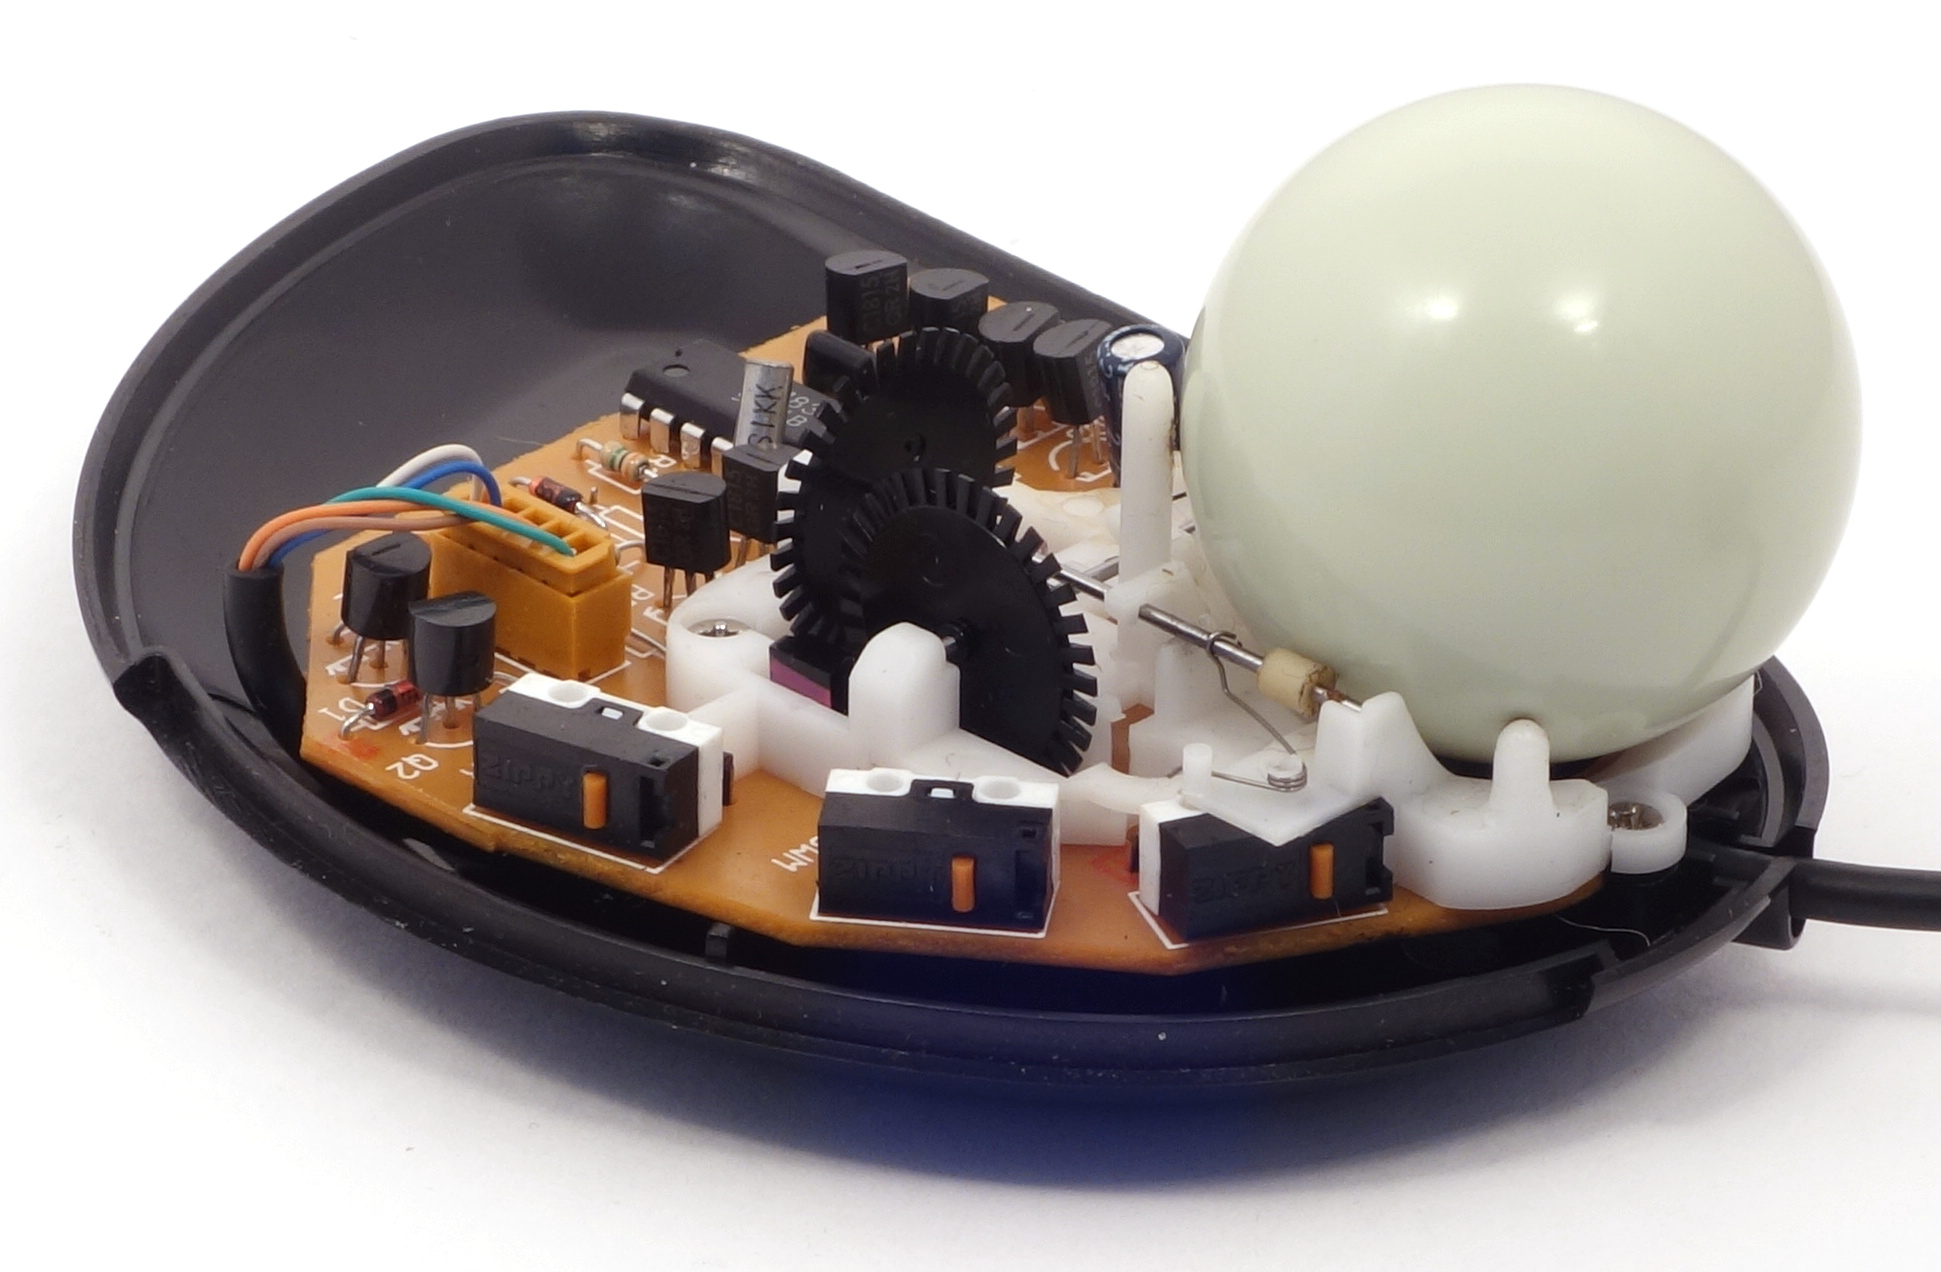
\includegraphics[scale=0.8]{1993_colani_trackball/inside_30.jpg}
    \caption{Colani Trackball disassembled}
    \label{fig:ColaniInside}
\end{figure}

\begin{thebibliography}{9}
    \bibitem {wiki} Luigi Colani – Wikipedia \url{https://en.wikipedia.org/wiki/Luigi_Colani}
    \bibitem {award} iF – HIGHSCREEN Colani Trackball \url{https://ifdesign.com/en/winner-ranking/project/highscreen-colani-trackball/19311}
\end{thebibliography}

\end{document}
